\documentclass[10pt]{article}
\usepackage[a4paper]{geometry}
\usepackage[usenames]{color} %used for font color
\usepackage{amssymb} %maths
\usepackage{amsmath} %maths
\usepackage{hyperref}
\usepackage[utf8]{inputenc} %useful to type directly diacritic characters
\usepackage{graphicx}
\begin{document}
\section{LHC luminosity}
%
\subsection{LHC parameters}
The circumference of the LHC ring is $l_{\rm LHC}=26659\,{\rm m}$ and the revolution time of the protons is $t_{\rm rev}=88.924\,\mu{\rm s}$ and the revolution frequency is $f_{\rm rev}=11245\,{\rm Hz}$. In an orbit there are slots for 3564 bunches separated by $\Delta t_{\rm bunch} = t_{\rm rev}/3564 = 24.95\,{\rm ns}$ and the bunch frequency is $f_{\rm bunch} = 3564\,f_{\rm rev} \simeq 40\,{\rm MHz}$.
%
\subsection{LHC luminous region}
\label{sec:lr}
The probability of an interaction per unit of volume and time is given by (\cite{bib:LandauFT}):
\begin{equation}
dn = \sqrt{({\bf v}_1-{\bf v}_2)^2-({\bf v}_1\times{\bf v}_2)^2/c^2}n_1n_2\sigma dVdt
\end{equation}
where ${\bf v}_1$ and ${\bf v}_2$ are the velocity of the incoming particles in the two beams, $\sigma$ is the cross section of the process under study, and $n_1$ and $n_2$ are the density of the particles in the two colliding beams.
In the approximation of two identical 3d gaussian distributions for the particle densities in the two beams, $n_1$ and $n_2$ are given by:
\begin{eqnarray}
n_1&=&\frac{N_{p_{bunch}}}{(2\pi)^{2/3}\sigma_x\sigma_y\sigma_z}e^{-\frac{x_1^2}{2\sigma_x^2}}e^{-\frac{y_1^2}{2\sigma_y^2}}e^{-\frac{(z_1-ct)^2}{2\sigma_z^2}} \\
n_2&=&\frac{N_{p_{bunch}}}{(2\pi)^{2/3}\sigma_x\sigma_y\sigma_z}e^{-\frac{x_2^2}{2\sigma_x^2}}e^{-\frac{y_2^2}{2\sigma_y^2}}e^{-\frac{(z_2+ct)^2}{2\sigma_z^2}}
\end{eqnarray}
where $\sigma_x,\,\sigma_y,\,\sigma_z$ are the RMS of the bunch in the two transverse directions and in the longitudinal directions and $N_{p_{bunch}}$ is the number of protons in the bunch. The coordinate systems $(x_{1,2},y_{1,2},z_{1,2})$ have been chosen with $z_{1,2}$ along the bunch longitudinal direction, parallel to the velocity for beam 1 and anti-parallel for beam 2, and with $x_{1,2}$ and $y_{1,2}$ in the transverse directions ($x$ horizontal and $y$ vertical).
If the two beams collide at an angle $2\alpha$ in the horizontal plane the two coordinates systems are related to the global coordinate systems $(x,y,z)$ according to:
\begin{eqnarray}
x_1 = x\cos\alpha - z\sin\alpha && x_2 = x\cos\alpha + z \sin\alpha\cr
y_1 = y && y_2 = y\cr
z_1 = z\cos\alpha + x\sin\alpha && z_2 = z\cos\alpha - x \sin\alpha
\end{eqnarray}
As a consequence the product $n_1n_2$ can be expressed as:
\begin{eqnarray}
n_1n_2&=&\frac{N^2_{p_{bunch}}}{(2\pi)^3\sigma_x^2\sigma_y^2\sigma_z^2}\exp\left({-\frac{x^2\cos^2\alpha}{2(\sigma_x/\sqrt{2})^2}}\right)
\exp\left({-\frac{y^2}{2(\sigma_y/\sqrt{2})^2}}\right)\cr
&&\exp\left({-\frac{z^2\cos^2\alpha}{2(\sigma_z/\sqrt{2})^2}\left(1+\frac{\sigma^2_z}{\sigma^2_x}\tan^2\alpha\right)}\right)
\exp\left({-\frac{c^2(x\sin\alpha/c-t)^2}{2(\sigma_z/\sqrt{2})^2}}\right)\\
&=&\frac{N^2_{p_{bunch}}}{(2\pi)^3\sigma_x^2\sigma_y^2\sigma_z^2}\exp\left({-\left(x-\frac{ct(\sigma^2_x/\sigma^2_z)\sin\alpha}{\cos^2\alpha+(\sigma^2_x/\sigma^2_z)\sin^2\alpha}\right)^2\frac{\cos^2\alpha}{2(\sigma_x/\sqrt{2})^2}\left(1+\frac{\sigma^2_x}{\sigma^2_z}\tan^2\alpha\right)}\right)\cr
&&\exp\left({-\frac{y^2}{2(\sigma_y/\sqrt{2})^2}}\right)\exp\left({-\frac{z^2\cos^2\alpha}{2(\sigma_z/\sqrt{2})^2}\left(1+\frac{\sigma^2_z}{\sigma^2_x}\tan^2\alpha\right)}\right)\cr
&&\exp\left({-\frac{c^2t^2}{2(\sigma_z/\sqrt{2})^2\left(1+\frac{\sigma^2_x}{\sigma^2_z}\tan^2\alpha\right)}}\right)
\end{eqnarray}
%
\subsection{Luminosity formula and reference value(s)}
LHC, and in general any collider with bunched beams luminosity, luminosity of heads-on collisions depends on the beam parameters according to the formulas below (all equivalent among each others):
\begin{equation}
{\cal L} = \frac{f_{\rm rev}N_{\rm bunches}N_{\rm p_{bunch}}^2}{4\pi\sigma_x\sigma_y}
= \frac{f_{\rm rev}N_{\rm p_{beam}}^2}{N_{\rm bunches}4\pi\sigma_x\sigma_y}
\label{LHClumi}
\end{equation}
where:
\begin{itemize}
\item $N_{\rm bunches}$ is the number of colliding bunches in LHC. In 2018 $N_{\rm bunches}=2544$ 
\item $N_{\rm p_{bunch}}$ is the number of protons per bunches, typically $1.1\cdot 10^{11}$ 
\item $N_{\rm p_{beam}} = N_{\rm bunches}\times N_{\rm p_{bunch}}$ is the number of protons per beam ($1.1\cdot 10^{11} \times 2544 \simeq 2.8\cdot 10^{13}$ equivalent to a current of $eN_{\rm p_{beam}}f_{\rm rev} \simeq 0.5 {\rm A}$)
\item $4\pi\sigma_x\sigma_y$ is the result of the integration of the luminous region (\ref{sec:lr}) in the gaussian approximation and $\sigma_x$ and $\sigma_y$ are the RMS of the beam distribution in the transverse directions. Typical values are $\sigma_{x,y}\simeq 10\,\mu{\rm m}$.\marginpar{To be expanded with the link with the emittance and the $\beta^*$ value}
\end{itemize}
With the parameter values proposed above the resulting LHC peak luminosity is:
\begin{equation}
{\cal L}_{\rm 2018ref}=\frac{11245\cdot 2544\cdot 1.21\cdot 10^{22}}{4\pi\cdot 10^{-6}}\,{\rm cm^{-2}s^{-1}} = 2.75\cdot 10^{34}\,{\rm cm^{-2}s^{-1}}
\end{equation}
%
\subsection{Single bunch crossing luminosity and event pileup}
Because of the bunched structure of the LHC beams and the fact that the detectors read out the collision events synchronised with the bunch crossings, one important parameter of the LHC is the luminosity integrated during one bunch crossing (BX) and that is expressed by the following formula:
\begin{equation}
\int_{\rm BX}{\cal L}\,{\rm dt} = \frac{{\cal L}}{N_{\rm bunches}f_{\rm rev}} = \frac{1}{N_{\rm bunches}f_{\rm rev}}\frac{f_{\rm rev}N_{\rm bunches}N_{\rm p_{bunch}}^2}{4\pi\sigma_x\sigma_y} = \frac{N_{\rm p_{bunch}}^2}{4\pi\sigma_x\sigma_y}
\end{equation}
With the parameter values proposed above the resulting integrated luminosity is:
\begin{equation}
\int_{\rm BX}{\cal L}\,{\rm dt}_{\rm 2018ref} = \frac{1.21\cdot 10^{22}}{4\pi\cdot 10^{-6}}\,{\rm cm^{-2}} = 0.96\,{\rm mb^{-1}}
\end{equation}
while, if the instantaneous luminosity is $2\cdot 10^{34}\,{\rm cm^{-2}s^{-1}}$, the integrated luminosity is:
\begin{equation}
\int_{\rm BX}{\cal L}\,{\rm dt}_{2\cdot 10^{34}} = \frac{2\cdot 10^{34}}{11245\cdot 2544}\,{\rm cm^{-2}} = 0.70\,{\rm mb^{-1}}
\end{equation}
Finally, being the inelastic pp cross section at 13\,TeV $\sigma_{\rm inel}=80\,{\rm mb}$ the number of pp collisions per bunch crossing, also known as event pileup (PU), for the two cases above, is:
\begin{eqnarray}
PU_{\rm 2018ref}&=&0.96\times 80 = 76.8\\
PU_{2\cdot 10^{34}}&=&0.7\times 80 = 56
\end{eqnarray}
\subsection{History of the LHC luminosity}
The peak luminosity achieved at the LHC in the past years is shown in figure~\ref{fig:peakLHC} \cite{LHCLumiInCMS}.
\begin{figure}[htbp]
\begin{center}
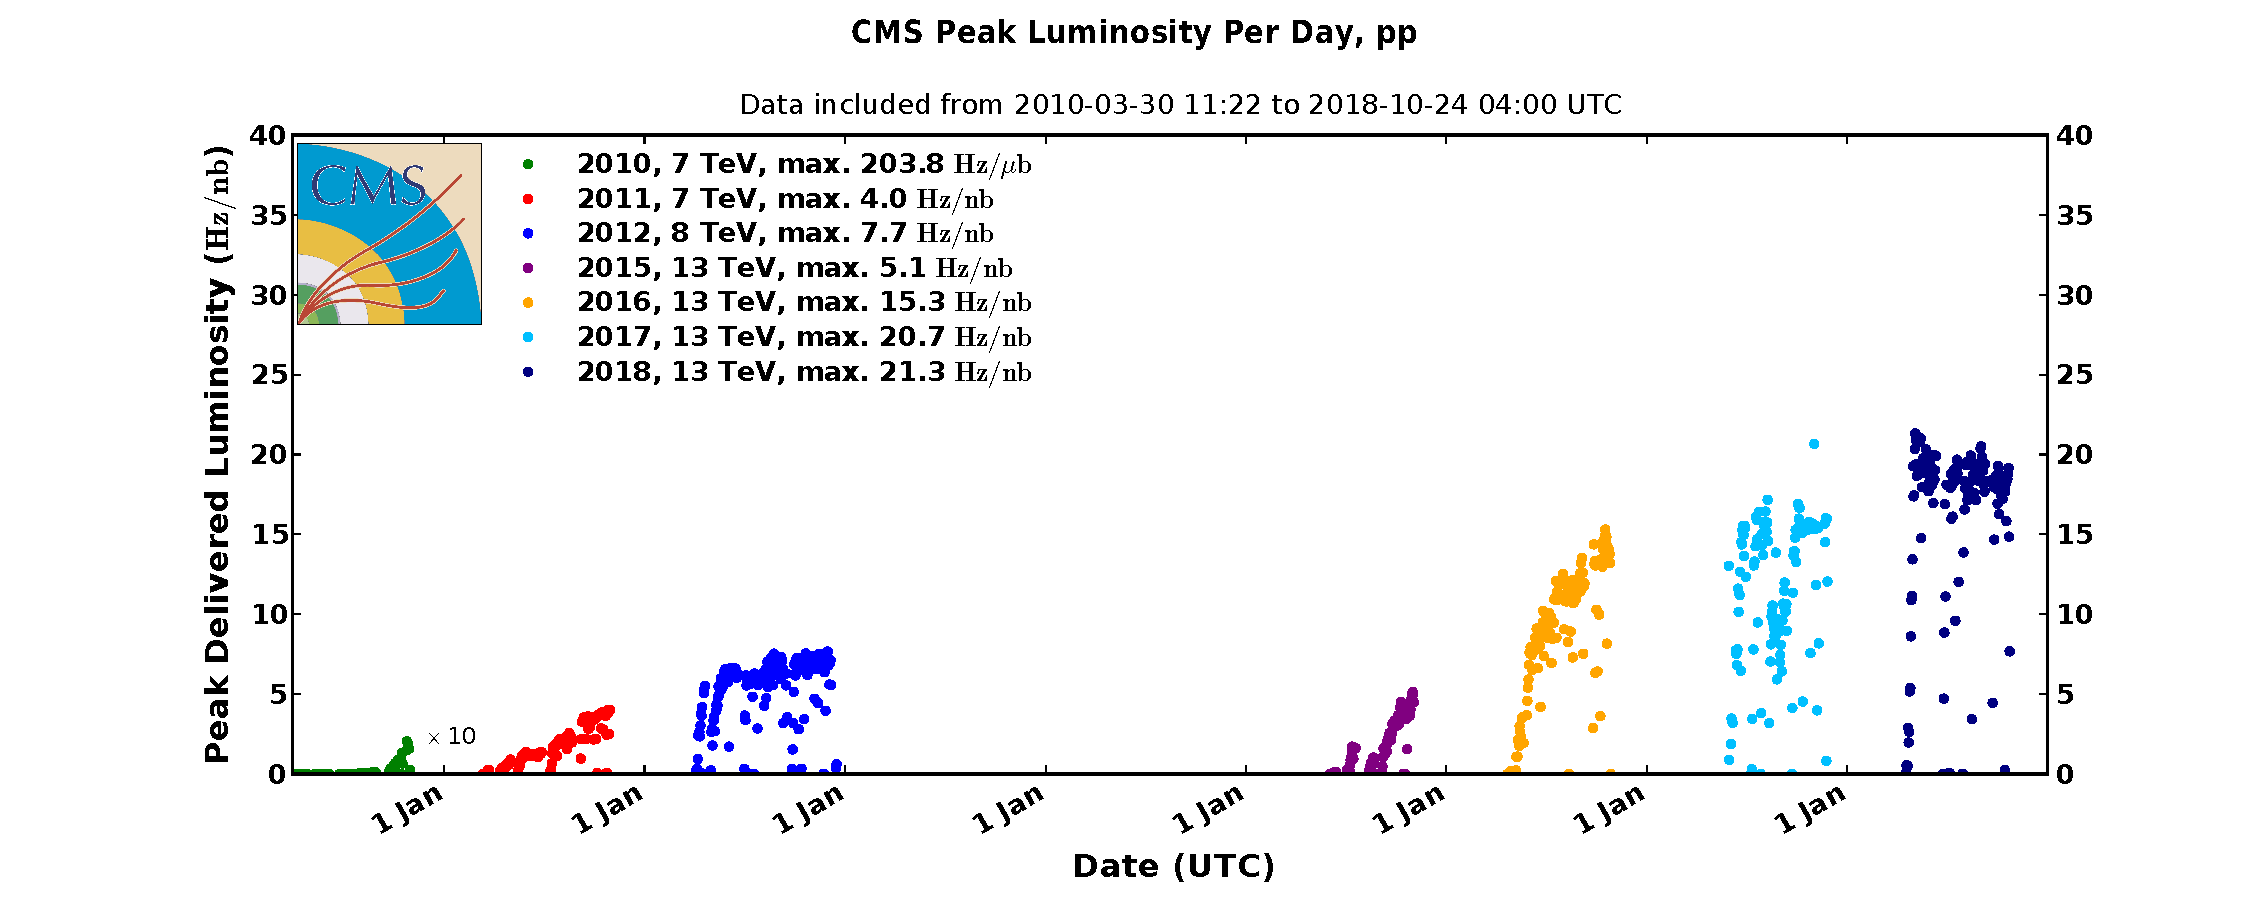
\includegraphics[width=\textwidth]{peak_lumi_pp.pdf}
\caption{{Peak luminosity versus time for 2010-2012 and 2015-2018}}
\label{fig:peakLHC}
\end{center}
\end{figure}
The delivered luminosity at the LHC in the past years is shown in figure~\ref{fig:deliveredLHC}
\begin{figure}[htbp]
\begin{center}
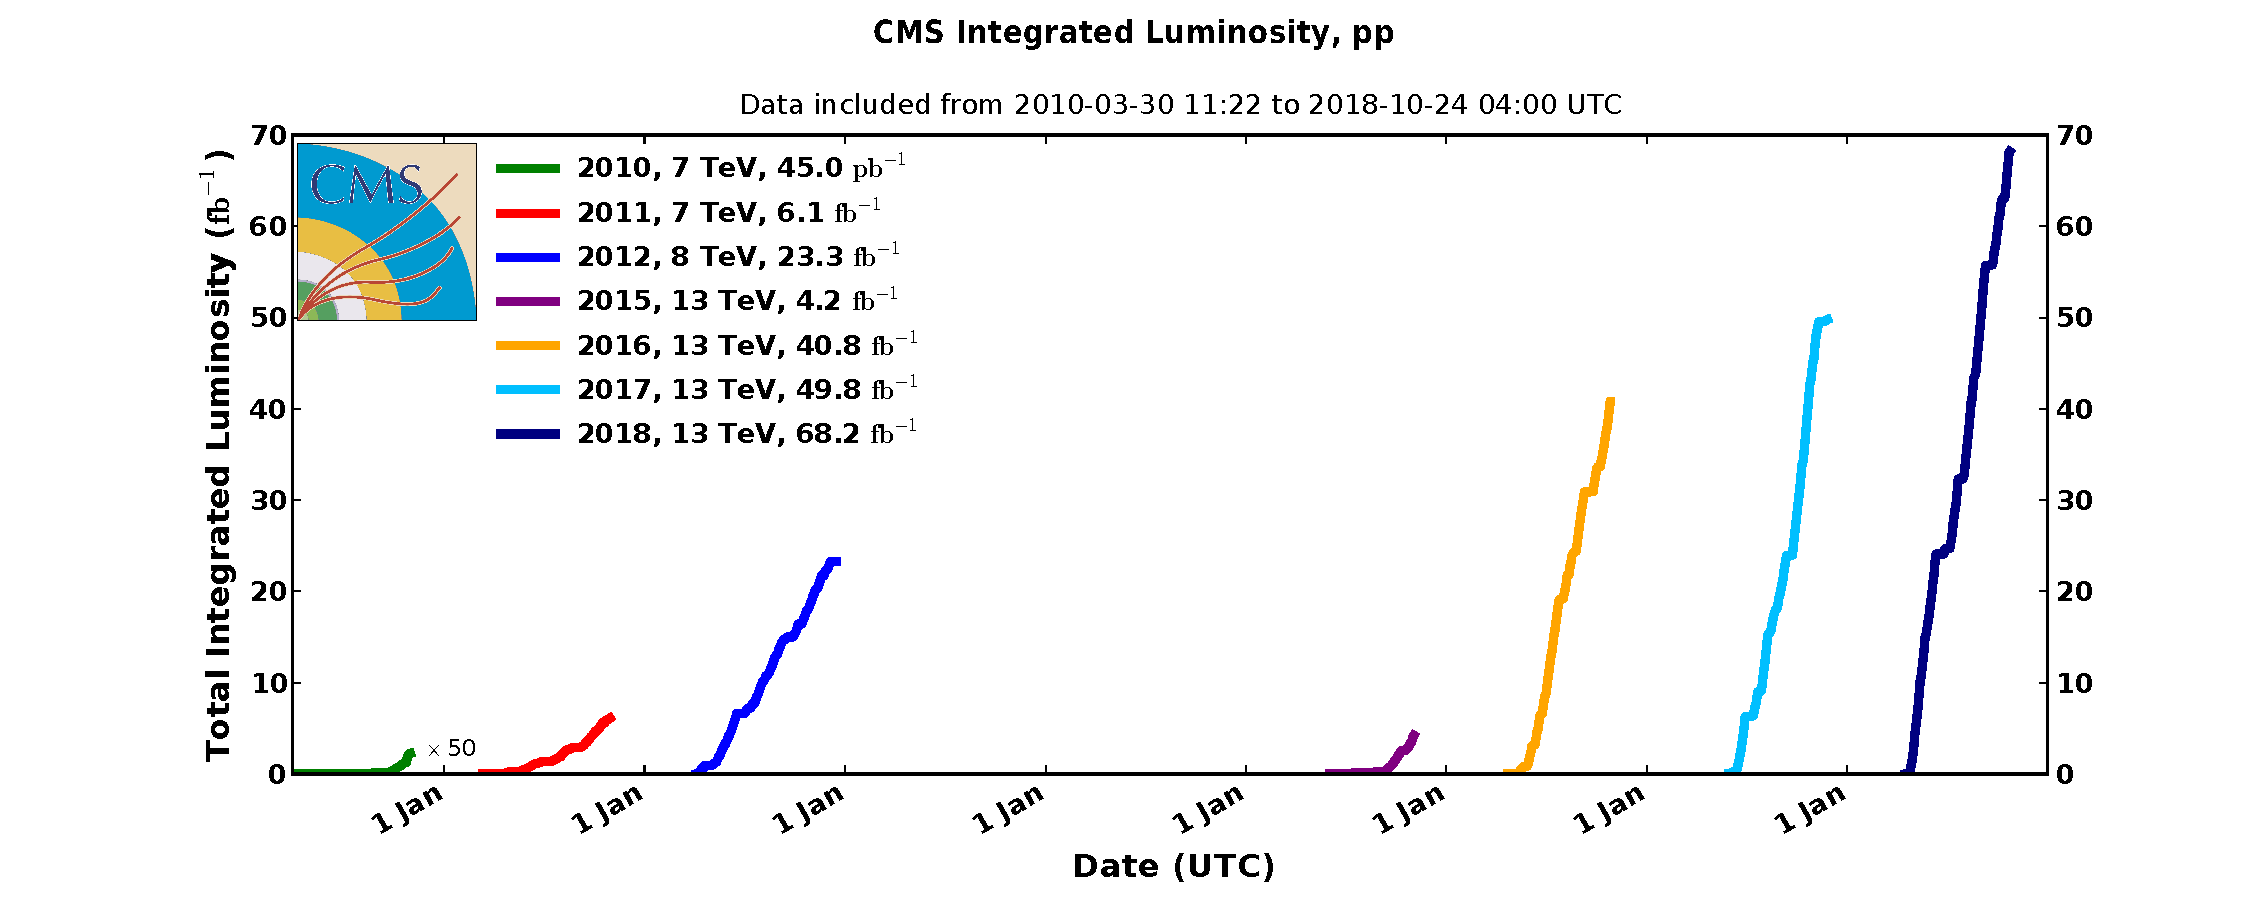
\includegraphics[width=\textwidth]{int_lumi_cumulative_pp.pdf}
\caption{{Delivered luminosity versus time for 2010-2012 and 2015-2018}}
\label{fig:deliveredLHC}
\end{center}
\end{figure}

%
\subsection{LHC luminosity lifetime}
The LHC proton beams loose protons for several reasons. One of them is the fact that protons collide and leave the beam or disintegrate. The rate of collisions and, therefore, the change of the number of protons in both beams depends on the total pp cross section ($\sigma_{\rm tot} \simeq 100\,{\rm mb}$ at 13\,TeV), on the number of interaction points ($N_{\rm int}$) and on the luminosity as follow:
\begin{equation}
\frac{dN_{\rm coll}}{dt} = N_{\rm int}{\cal L}\sigma_{\rm tot}\ \Rightarrow\ \frac{dN_{\rm p_{beam}}}{dt} = - N_{\rm int}{\cal L}\sigma_{\rm tot}
\end{equation}
Using one of the formulas (\ref{LHClumi}), the rate of change of the number of protons in the beams can be transformed into the following differential equation:
\begin{equation}
\frac{dN_{\rm p_{beam}}}{dt} = - N_{\rm int}\sigma_{\rm tot} \frac{f_{\rm rev}}{N_{\rm bunches}4\pi\sigma_x\sigma_y}N_{\rm p_{beam}}^2
\end{equation}
whose solution is:
\begin{equation}
N_{\rm p_{beam}}(t) = \frac{1}{\frac{N_{\rm int}\sigma_{\rm tot}f_{\rm rev}}{N_{\rm bunches}4\pi\sigma_x\sigma_y}t+\frac{1}{N^0_{\rm p_{beam}}}} = \frac{{N^0_{\rm p_{beam}}}}{\frac{N_{\rm int}{\cal L}^0\sigma_{\rm tot}}{{N^0_{\rm p_{beam}}}}t+1}
\end{equation}
As a consequence, the luminosity depends on time in the following way:
\begin{equation}
{\cal L}(t) = \frac{f_{\rm rev}N_{\rm p_{beam}}^2(t)}{N_{\rm bunches}4\pi\sigma_x\sigma_y} = 
\frac{{\cal L}^0}{\left(\frac{N_{\rm int}{\cal L}^0\sigma_{\rm tot}}{N^0_{\rm p_{beam}}}t+1\right)^2}
\label{lumivstime}
\end{equation}
and the time $t_{1/2}$ after which the luminosity is reduced to half of its peak value is given by:
\begin{equation}
t_{1/2} = (\sqrt{2}-1)\frac{N^0_{\rm p_{beam}}}{N_{\rm int}{\cal L}^0\sigma_{\rm tot}} = (\sqrt{2}-1)\frac{N_{\rm bunches} 4\pi\sigma_x\sigma_y}{N_{\rm int}\sigma_{\rm tot}N^0_{\rm p_{beam}}f_{\rm rev}}
\end{equation}
If ${\cal L}^0=2\cdot 10^{34}\,{\rm cm^{-2}s^{-1}}$, $N_{\rm int}=2$, and $N_{\rm p_{beam}} = 2544\times 1.1\cdot 10^{11}$:
\begin{equation}
t_{1/2_{2\cdot 10^{34}}} = (\sqrt{2}-1)\frac{2544\times 1.1\cdot 10^{11}}{2\times 2\cdot 10^{34}\times 100\cdot 10^{-27}}\,{\rm s} = 0.290 \cdot 10^5\,{\rm s}\simeq 8\,{\rm hours}
\end{equation}
In figure~\ref{fig:lumivstime} the trend resulting from (\ref{lumivstime}) (top plot) and the observed trend in one LHC fill (bottom plot) are shown. The actual time needed to reduce the luminosity by 50\% is about 8 hours, as expected.
\begin{figure}[htbp]
\begin{center}
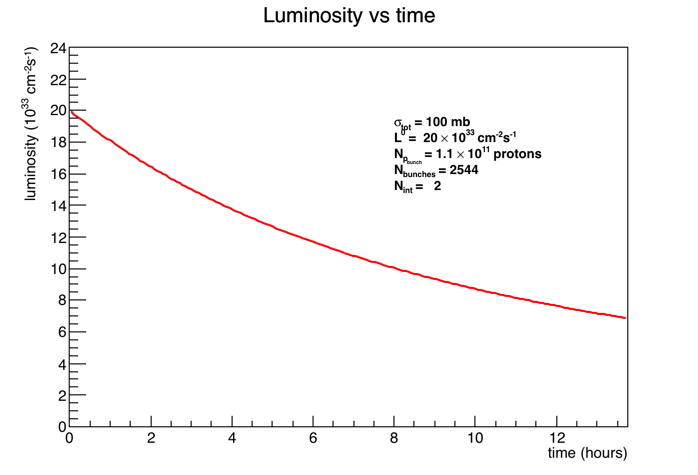
\includegraphics[width=\textwidth]{lumivstime.png}
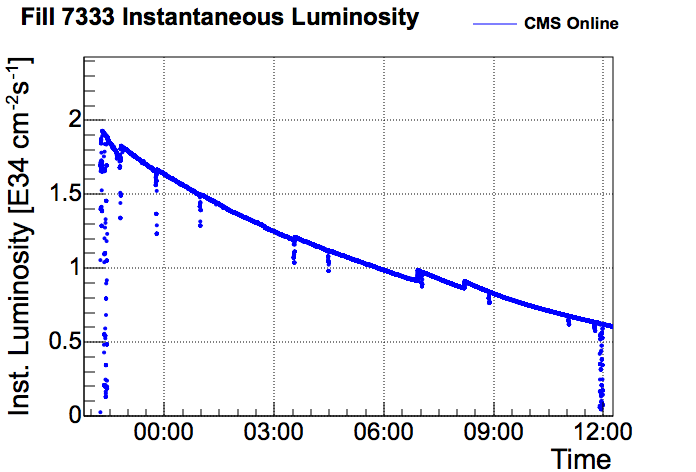
\includegraphics[width=\textwidth]{fill_7333_inst_lumi_cms.png}
\caption{Expected time dependence of the luminosity if the collisions are the only cause of beam losses (top plot) and observed time dependence of the luminosity in one LHC fill (bottom plot)}
\label{fig:lumivstime}
\end{center}
\end{figure}

%
\begin{thebibliography}{1}
\bibitem{bib:LandauFT} Landau, Teoria dei Campi
\bibitem{LHCLumiInCMS} CMS Luminosity Public Results \href{url}{https://twiki.cern.ch/twiki/bin/view/CMSPublic/LumiPublicResults}
\end{thebibliography}



\end{document}